\documentclass[12pt]{article}
\usepackage{fullpage,graphicx,psfrag,amsmath,amsfonts,verbatim}
\usepackage{listings, color}
\definecolor{mygreen}{rgb}{0,0.6,0}
\definecolor{mygray}{rgb}{0.5,0.5,0.5}
\definecolor{mymauve}{rgb}{0.58,0,0.82}
\usepackage[scaled]{beramono}
\usepackage{courier, natbib}
\usepackage[usenames,dvipsnames]{xcolor}
\usepackage{hyperref, adjustbox}
\usepackage[small,bf]{caption}
\usepackage{float}
\usepackage{booktabs}

\newcommand{\subf}[2]{%
  {\small\begin{tabular}[t]{@{}c@{}}
  #1\\#2
  \end{tabular}}%
}

\lstset{
  language=Python,
  backgroundcolor=\color{white},
  breaklines=true,
  captionpos=b,
  commentstyle=\color{mygreen},
  showstringspaces=false,
  formfeed=newpage,
  keepspaces=true,
  stringstyle=\color{mymauve},
  keywordstyle=\color{blue},
  numbers=left,
  tabsize=4,
  numberstyle=\footnotesize,
  basicstyle=\footnotesize,
  morekeywords={models, lambda, forms, True, False, self}
}

\newcommand{\code}[2] {
  \hrulefill
  \subsection*{#1}
  \lstinputlisting{#2}
  \vspace{2em}
}

\newcommand{\tab}[1]{\hspace{.2\textwidth}\rlap{#1}}

\input defs.tex

\title{\texttt{CompleteThat}: A python package for  low-rank matrix completion}
\author{Joshua Edgerton \and Esteban Fajardo}
\date{January 5, 2014}

\begin{document}

\maketitle

\begin{abstract}
We have developed a Python package (\texttt{CompleteThat}) to perform low rank matrix completion. Given a low rank matrix with partial entries we implemented different methods to solve the matrix completion problem:  First, for ``small'' problems we implemented two memory-based algorithms  following the work by Tanner and Wei~\cite{Tanner:2014} to find, given a number $r$, the matrix with rank $r$ that best fits the data using the Frobenius norm. Second, when the problem does not fit into memory, we implemented a memory-fitting algorithm (stochastic gradient descent) following the approach in Zhang~\cite{zhang:2004} and Bottou~\cite{bottou:2012}. The package is available at \url{https://pypi.python.org/pypi/completethat/0.1dev}. 
\end{abstract}

\newpage
\tableofcontents
\newpage

\section{Introduction}
Matrix factorization has recently seen a large growth in popularity within the mathematics, statistics, and computer science communities as industry continues to apply machine learning techniques on a wide array of problems and scenarios. For our convex optimization project, we decided to take some of the more interesting and applicable topics and algorithms of our class and develop a python package to implement them. We briefly discuss the theory behind matrix factorizing, the models and approaches we choose to use and the algorithms for the optimization. Later, we walk through two case studies illustrating the usefulness and applicability in the context of image processing and a recommendation system for Yahoo music and movie data. 

\section{Matrix Completion Problem}
The matrix completion problem can be formally stated as follows. We are interested in recovering a matrix $M \in \reals^{n_1 \times n_2}$ but only get to observe a number $m \ll n_1n_2$ of its entries. Thus, we want to find a solution to the following optimization problem

\begin{equation}
    \begin{array}{ll}
    \mbox{minimize}   &  \rank(X)\\
    \mbox{subject to} & X_{ij} = M_{ij} \qquad (i,j)\in \Omega
    \end{array}
    \label{eq:original_problem1}
\end{equation}
where $X\in \reals^{n_1 \times n_2}$ is the decision variable and $\rank(X)$ is equal to the rank of the matrix $X$. The problem (\ref{eq:original_problem1}) seeks the simplest matrix fitting the observed data. Of course, if there were only one low-rank object fitting the data, this would recover $M$.  
In order to fix the notation correctly define the projector $P_{\Omega}:\reals^{n_1\times n_2} \rightarrow \reals^{n_1\times n_2} $ as

\begin{equation*}
P_{\Omega}(A) = \left \{ 
	\begin{array}{lr}
		A_{ij} & : (i,j) \in \Omega\\
		0 & : \mathrm{otherwise}
	\end{array}
	\right.
\end{equation*}\\
Using the projector, Problem (\ref{eq:original_problem1}) can be rewritten as
\begin{equation}
    \begin{array}{ll}
    \mbox{minimize}   &  \rank(X)\\
    \mbox{subject to} & P_{\Omega}(X) = P_{\Omega}(M)
    \end{array}
    \label{eq:original_problem2}
\end{equation}

Unfortunately, this optimization problem has been shown to be NP-hard and all know algorithms which provide exact solutions require time doubly exponential in the dimension of the matrix both in theory and in practice~\cite{Candes:2009}. Also, the $\rank(X)$ makes the problem non-convex. 

Several approximations to the problem exists. One, the ``tightest convex relaxation of $\rank(X)$''~\cite{Fazel:2002} is the following problem

\begin{equation}
    \begin{array}{ll}
    \mbox{minimize}   &  \|X\|_* :=\sum_{i=1}^r \sigma_i(X) \\
    \mbox{subject to} & P_{\Omega}(X) = P_{\Omega}(M)
    \end{array}
    \label{eq:nucl_problem}
\end{equation}

where $\sigma_i(X)$ denotes the $i$th largest singular value of $X$ and $\|X\|_*$ is the called the nuclear norm. The main point of this relaxation is that the nuclear norm is a convex function and thus can be optimized efficiently via semidefinite programming or by iterative soft thresholding algorithms~\cite{cai:2010}~\cite{goldfarb:2011}.

Alternative to nuclear norm minimization there have been many algorithms which are designed to target the following optimization problem
\begin{equation}
    \begin{array}{ll}
    \mbox{minimize}_{Y,Z}   & \frac{1}{2} \|P_{\Omega}(YZ) - P_{\Omega}(M)\|^2_F \\
    \end{array}
    \label{eq:frob_problem}
\end{equation}
where $X=YZ$ is the completed matrix and $Y\in \reals^{n_1\times r}, Z\in \reals^{r\times n_2}$ and $r$ represents the (hopefully small) rank of the matrix $X$.

\section{Implementation}
\texttt{CompleteThat} is a python package that solves the low rank matrix completion problem. Given a low rank matrix with partial entries the package solves an optimization problem to estimate the missing entries. We allow the user to choose between several optimization algorithms including two in memory based algorithms, alternating steepest descent and scaled alternating steepest descent, and one out of memory fitting procedure using stochastic gradient descent. We use extensively the numerical libraries \texttt{spicy} and \texttt{numpy}, and the current implementation includes two classes, \texttt{MatrixCompletion} for in memory based algorithms and \texttt{MatrixCompletionBD} for the memory fitting procedure. The package is available worldwide and can be
downloaded from \url{https://pypi.python.org/pypi/completethat/0.1dev}.

\subsection*{CVX}
Problem (\ref{eq:nucl_problem}) can be easily solved directly using CVX, a package for specifying and solving convex programs~\cite{cvx}, ~\cite{gb08}, with the following code:

\begin{verbatim}
index = find(~isnan(M));
cvx_begin
    variable X(size(M));
    minimize norm_nuc(X)
    % s.t.
    X(index) == M(index);
cvx_end
\end{verbatim}

Where M is a MATLAB matrix with nan on the missing entries and \texttt{X(index) == M(index)} corresponds to the $P_{\Omega}(X) = P_{\Omega}(M)$ restriction. However, the computation is very slow and for any matrix greater than 100x100 the computational time is too high. Since this is clearly unsatisfactory for practical purposes, specific algorithms were implemented on the package. 

\subsection*{Algorithms}
\subsubsection*{Low rank matrix completion by alternating steepest descent methods}
\subsubsection*{Low rank matrix completion by stochastic gradient descent}

\subsection*{Code Example}
For matrices that fit into memory use the \texttt{MatrixCompletion} module. Otherwise, use \texttt{MatrixCompletionBD} module. 

\subsubsection*{MatrixCompletion}
Given a \texttt{numpy} matrix $M$ with \texttt{numpy.nan} on the missing entries, the matrix completion problem can be solved (using ASD) as:
\begin{verbatim}
>>> from completethat import MatrixCompletion
>>> problem = MatrixCompletion(M)
>>> problem.complete_it("ASD")
>>> X = problem.get_matrix() #Desired matrix
>>> out_info = problem.get_out() #Extra information
\end{verbatim}

\subsubsection*{MatrixCompletionBD}
Given a csv file with the input data, the matrix completion problem can be solved as:

\begin{verbatim}
>>> from completethat import MatrixCompletionBD
>>> problem = MatrixCompletionBD('input_data.txt')
>>> problem.train_sgd(dimension=6,init_step_size=.01,min_step=.000001, 
       reltol=.001,rand_init_scale=10, maxiter=1000,
       batch_size_sgd=50000,shuffle=True)
>>> problem.validate_sgd('test_data.txt')
>>> problem.save_model()
\end{verbatim}

\section{Case Studies}
\subsection*{Yahoo movies and music reviews database}
The Yahoo music and movie data sets are publicly available datasets published by Yahoo for use to the public for recreational and research purposes. The music training data set is a small 4 mb pipe-delimited file consisting of roughly 210,000 user-movie ratings. The test set has roughly 10,000 records. There are two ratings schemas available, one on a 5-point scale and the other on a 13-point scale and we arbitrarily chose to use the 5-point scale. The Yahoo music data is a larger 2.2 gb file of 115 million user-song ratings. The ratings are on a 100 point scale.
 
We look to evaluate the performance of our algorithms on these two datasets, comparing the various algorithms implemented versus a naive benchmark estimate where we used the mean of the training set as our estimator for all records in the test set. Then we compared how well the algorithms performed versus the benchmark. 

The benchmark for the yahoo music data is 4.088. This is the mean value of the ratings in the training set so we will compute the MSE on the test set using the benchmark which yields an RMSE of 1.10. A quick run of Mahout yields 1.17 and CompleteThat's sgd model yielded a 1.19. So our model yielded a pretty similar RMSE as the MAHOUT package. Note that for both of these instances we used a factorization of rank equal to seven and the Complete that sgd algorithm ran slightly faster than Mahout's (.537 minutes vs 1.4 minutes). 

\begin{table}[h]
\centering
\resizebox{0.75\textwidth}{!}{%
\begin{tabular}{@{}ccccc@{}}
\toprule
\multicolumn{1}{l}{\textbf{Step size}} & \multicolumn{1}{l}{\textbf{Iterations}} & \multicolumn{1}{l}{\textbf{Minutes}} & \multicolumn{1}{l}{\textbf{Train MSE}} & \multicolumn{1}{l}{\textbf{Test RMSE}} \\ \midrule
1 & 8 & 0.585 & 1.411 & 1.757 \\
2 & 8 & 0.598 & 1.304 & 1.550 \\
3 & 8 & 0.628 & 1.235 & 1.483 \\
4 & 8 & 0.617 & 1.180 & 1.397 \\
5 & 7 & 0.538 & 1.136 & 1.351 \\
6 & 7 & 0.534 & 1.100 & 1.244 \\
7 & 7 & 0.534 & 1.071 & 1.194 \\
8 & 7 & 0.541 & 1.046 & 1.127 \\
9 & 7 & 0.537 & 1.027 & 1.128 \\
10 & 7 & 0.529 & 1.010 & 1.102 \\
15 & 7 & 0.551 & 0.971 & 1.063 \\
20 & 7 & 0.540 & 0.976 & 1.075 \\
30 & 8 & 0.614 & 1.045 & 1.359 \\ \bottomrule
\end{tabular}
}
\caption{RMSE vs Step Size vs Rank}
\end{table}

\clearpage
\subsection*{Columbia University photographs}
In this section, we demonstrate the applicability of the package to image processing problems. By randomly erasing a predefined proportion of the pixels of an image the problem of completing the image can be cast as a matrix completion problem. For illustration we used three  512 x 512 grayscale photographs taken by one of the authors of the Columbia University campus on December, 2014. The reconstructed images can be seen on Figure~\ref{fig:columbia_pics}, where we erased 65\% of the pixels of each image. 

In addition, to illustrate the ease of use of the package we also present the script used to solve all the problems in what follows:

\lstinputlisting[numbers=none]{columbia_images.py}

\begin{figure}[H]
\resizebox{\textwidth}{!}{%
\makebox[\textwidth][c]
{
\begin{tabular}{ccc}
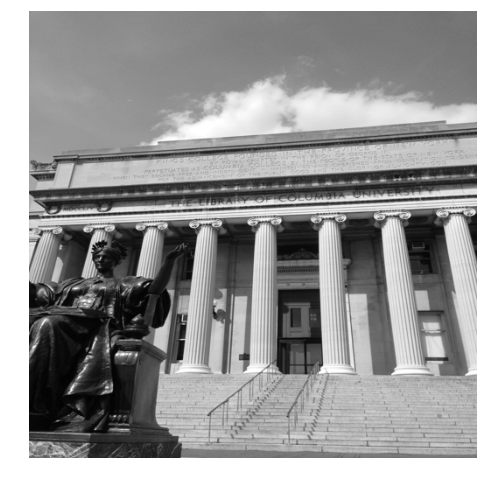
\includegraphics[width=65mm]{figures/columbia1.png}
&
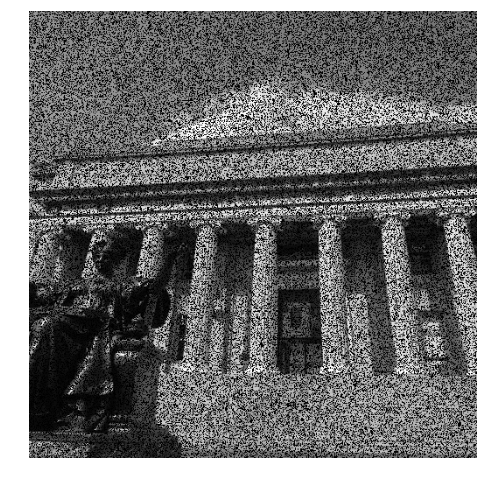
\includegraphics[width=65mm]{figures/columbia2.png}

&
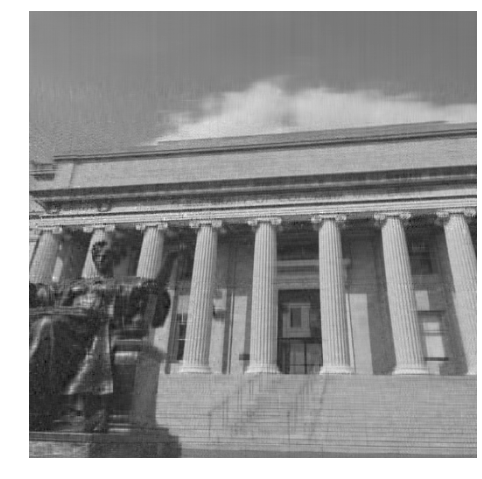
\includegraphics[width=65mm]{figures/columbia3.png}

\\

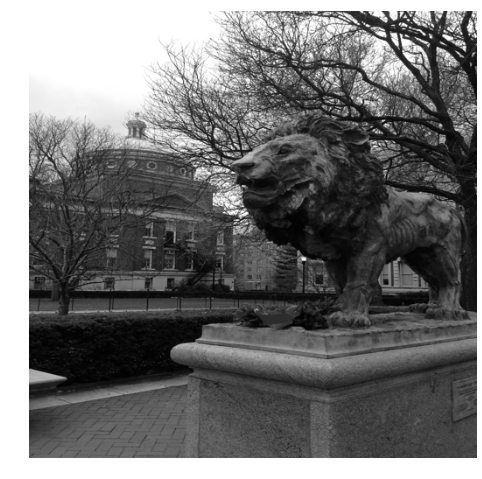
\includegraphics[width=65mm]{figures/columbia4.png}
&
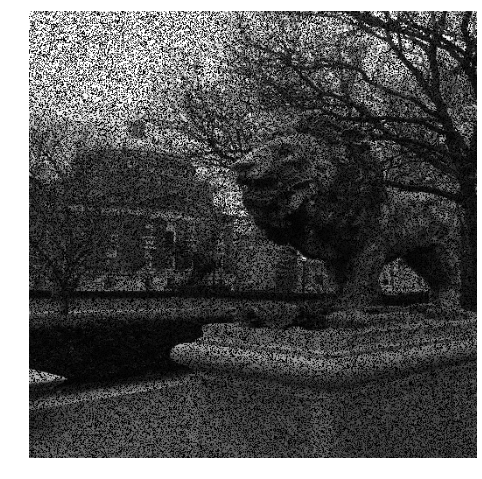
\includegraphics[width=65mm]{figures/columbia5.png}
&
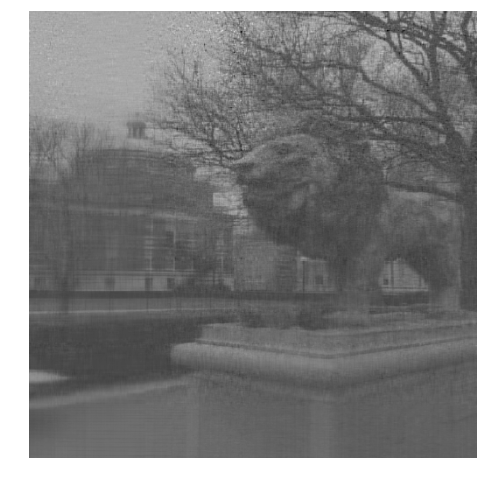
\includegraphics[width=65mm]{figures/columbia6.png}
\\

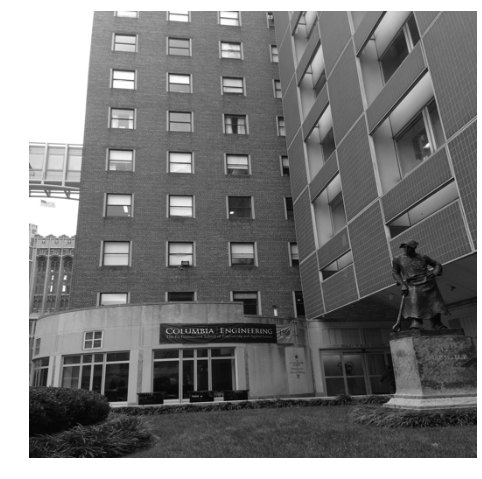
\includegraphics[width=65mm]{figures/columbia7.png}
&
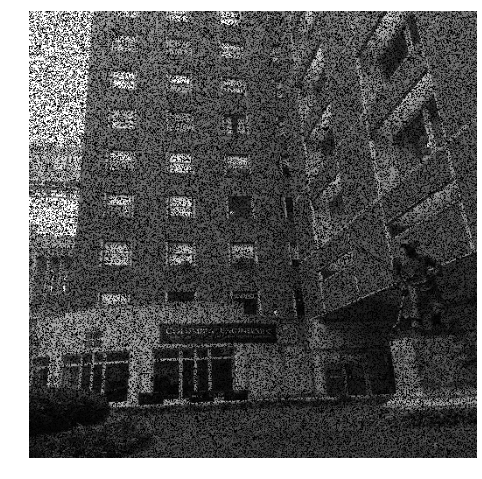
\includegraphics[width=65mm]{figures/columbia8.png}
&
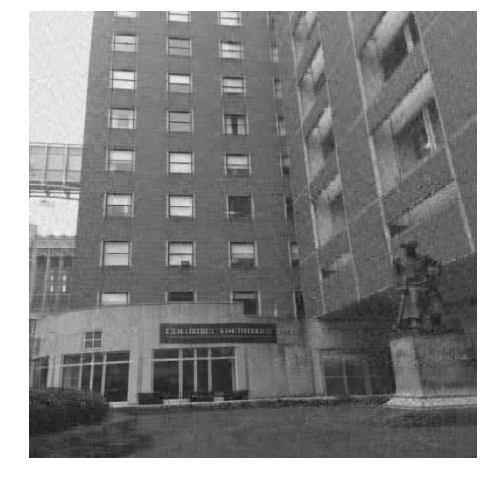
\includegraphics[width=65mm]{figures/columbia9.png}
\\
\end{tabular}
}
}

\caption{ASD method applied three different Columbia University photographs using random sampling}
\label{fig:columbia_pics}
\end{figure}

\section{Future Work}

We have plans for various improvements as we continue working with the \texttt{CompleteThat} python package. Overall, we would like to test the software and integrate automated testing cases into the software developing cycle. Also, documentation for the package and its functions, including examples, is high in our priority list. In addition, we hope to incorporate more rigorous error checking and make   available more customization to the user. 

For the memory-based algorithms it is well know that noise in the data introduces overfitting on the estimated matrix. Following the approach taken by Mazumder et al.~\cite{mazumder:2010}  where they solve the same objetive function as the problems above (using the Frobenious norm) but introducing the nuclear norm as regularizer to account for overfitting, we would introduce a regularization option into the matrix completion procedure. 

For the stochastic gradient descent method, we plan to add a lambda penalty feature for combatting overfitting as well as considering options for more advanced versions of our basic latent factor model as demonstrated by Koren~\cite{koren:2008} in his paper on the prize-winning Netflix models. 
For all algorithms, we would like to explore and research various hardware and software optimization techniques for faster code. 

Finally, given the similarities between matrix completion and robust principal component analysis one further extension to the functionality of the package could be implementing the robust-PCA procedure outlined by Cand\'es~\cite{candes:2011}, et al.

\newpage
\bibliographystyle{alpha}
\bibliography{references}

\newpage
\section{Source code}
On the whole, the package directory structure looks like the Figure~\ref{fig:code_scheme}. In the following we present the source code for the package.
\begin{figure}[h!]
  \centering
    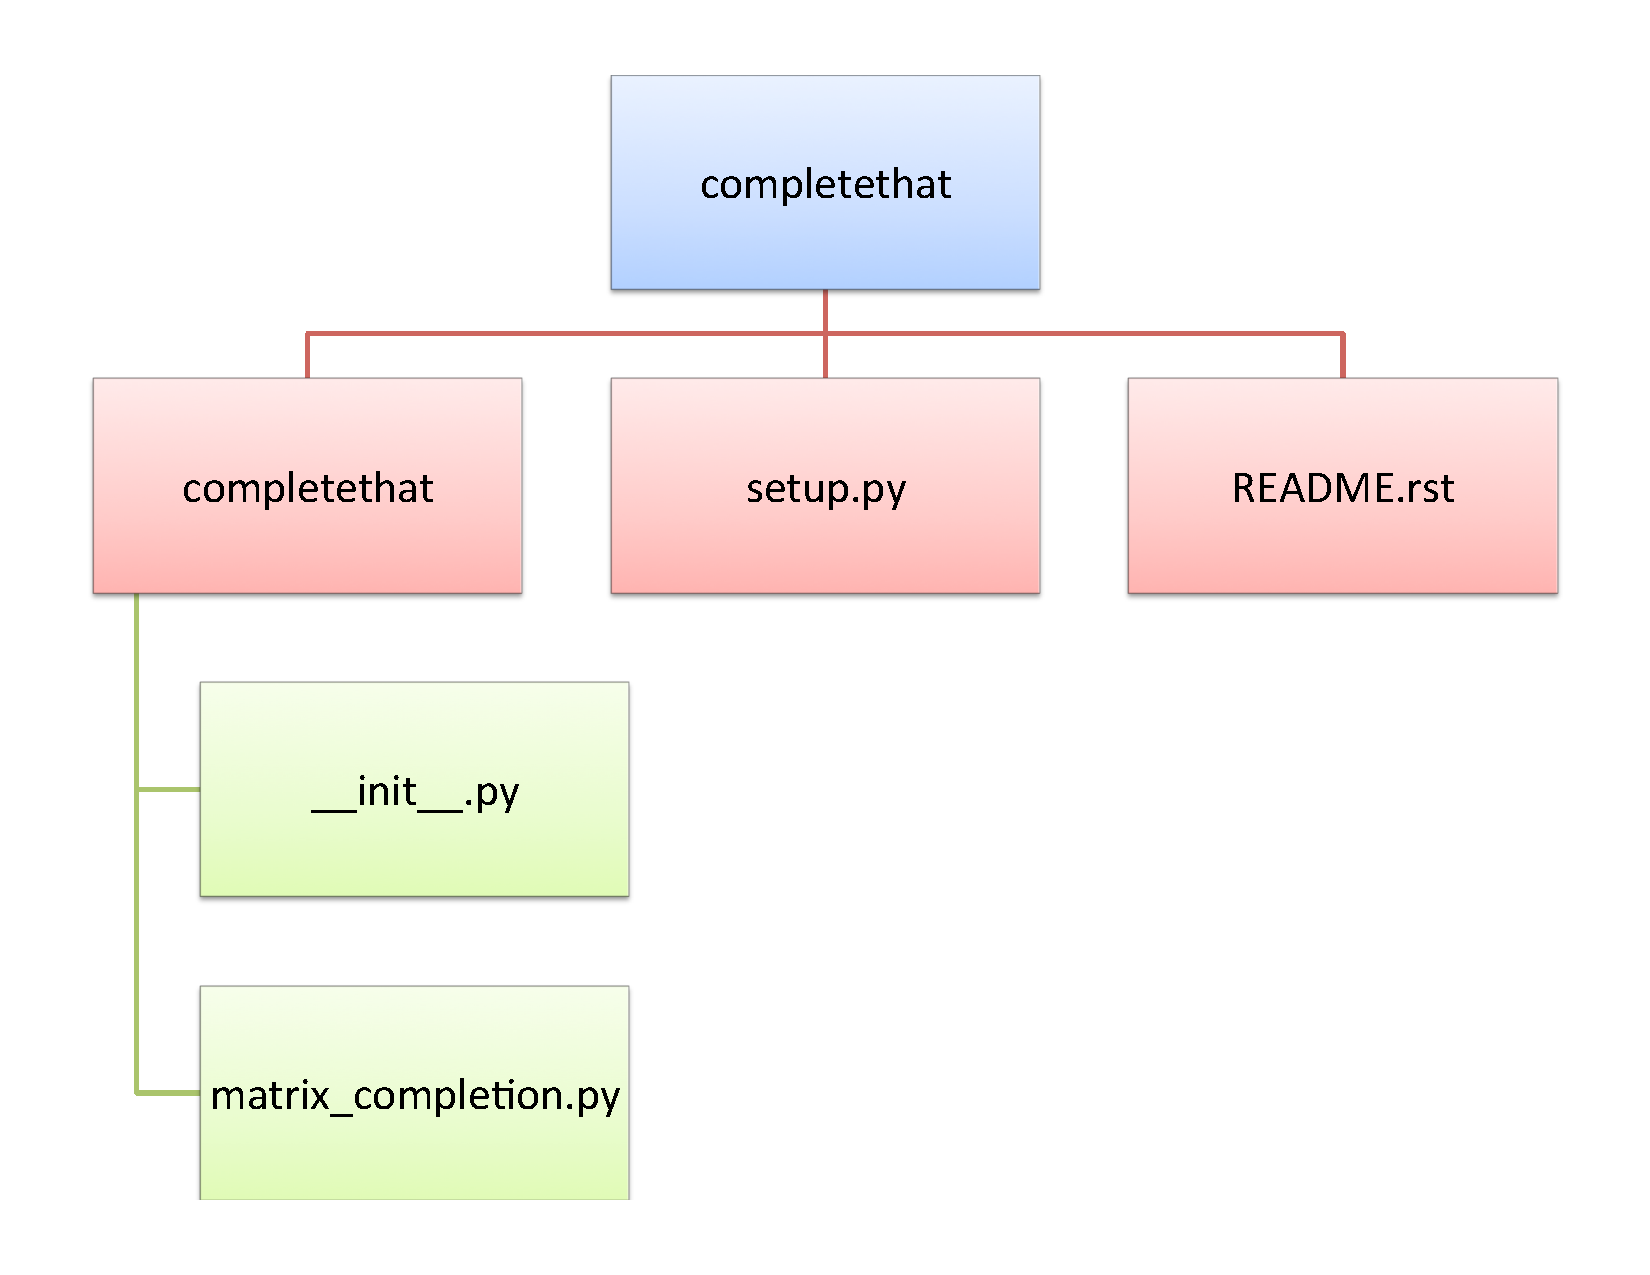
\includegraphics[width=0.8\textwidth]{./figures/code_scheme.pdf}
    \caption{CompleteThat structure}
    \label{fig:code_scheme}
\end{figure}

\code{completethat/matrix\_completion.py}{../code/completethat/matrix_completion.py}
\code{completethat/matrix\_\_init\_\_.py}{../code/completethat/__init__.py}
\code{completethat/matrix\_\_init\_\_.py}{../code/setup.py}


\end{document}